\chapter{The Standard Model}
    \label{chapter:StandardModel}

This chapter describes the main theoretical and phenomenological concepts of the Standard Model of particle physics, and the structure of the proton.
Monte Carlo simulations of Standard Model processes are also discussed in the following.


\section{Introduction to the Standard Model}
    \label{sec:IntroSM}

The Standard Model (SM) of particle physics \cite{Glashow:1961tr, Weinberg:1967tq, Salam:1980jd} is a renormalizable quantum field theory based on the total invariance under the gauge group

\begin{equation}
SU(3)_{c}\otimes SU(2)_{L}\otimes U(1)_{Y}
\label{eq:SMSymmetryGroup}
\end{equation}

\noindent that describes the properties of all the fundamental particles and the interactions among them.
The SM is divided into a bosonic and a fermionic sectors.
The bosonic sector of the SM is responsible for three of the four interactions in Nature.
Gravity cannot be accommodated, thus being one of the main motivations to look for physics beyond the Standard Model.
Table~\ref{tab:bosons} summarizes the boson classification of the SM.

\begin{table}[!ht]
  \begin{center}
    \begin{small}
      \setlength{\tabcolsep}{0.0pc}
      \begin{tabular*}{\textwidth}{@{\extracolsep{\fill}}lcccc}
        \noalign{\smallskip}\hline\noalign{\smallskip}
         {\bf Mediator}               & {\bf Mass [GeV]}     & {\bf Interaction} & {\bf Electric charge} & {\bf Spin} \\
        \noalign{\smallskip}\hline\noalign{\smallskip}
         Gluon ($\times 8$) $(g)$     & 0                    & strong            & 0                     & 1 \\
         Photon ($\gamma$)            & 0                    & electromagnetic   & 0                     & 1 \\
         $Z$                          & $91.1876 \pm 0.0021$ & weak (neutral)    & 0                     & 1 \\
         $W^{\pm}$                    & $80.385 \pm 0.015$   & weak (charged)    & $\pm 1$               & 1 \\
         Higgs ($H$)                  & $125.7 \pm 0.4$      & -                 & 0                     & 0 \\
        \noalign{\smallskip}\hline\noalign{\smallskip}
      \end{tabular*}
    \end{small}
  \end{center}
  \caption[Bosonic fields in the Standard Model.]{Boson classification in the Standard Model.}
  \label{tab:bosons}
\end{table}

The fermionic sector is composed of quarks and leptons, and is organized in three families (generations).
Generations only differ one to another by their mass.
Table \ref{tab:QuarksAndLeptons} provides a classification of the Standard Model quarks and leptons.

\begin{table}[!t]
  \begin{center}
    \begin{small}
      \setlength{\tabcolsep}{0.0pc}
      \begin{tabular*}{\textwidth}{@{\extracolsep{\fill}}l|ccc}
        \hline
        \textbf{SM fermions}     & \textbf{1st generation}         & \textbf{2nd generation}         & \textbf{3rd generation} \\
        \hline
        \multirow{4}{*}{QUARKS}  & Up (\textbf{u})                 & Charm (\textbf{c})              & Top (\textbf{t})\\
                                 & \tiny{charge = $+2/3$}          & \tiny{charge = $+2/3$}          & \tiny{charge = $+2/3$} \\
%        \cline{2-4}
& & & \\
                                 & Down (\textbf{d})               & Strange (\textbf{s})            & Bottom (\textbf{b})\\
                                 & \tiny{charge = $-1/3$}          & \tiny{charge = $-1/3$}          & \tiny{charge = $-1/3$} \\
        \hline
        \multirow{4}{*}{LEPTONS}& Electron neutrino ($\nu_e$)     & Muon neutrino ($\nu_\mu$)       & Tau neutrino ($\nu_\tau$)\\
                                 & \tiny{charge = $0$}             & \tiny{charge = $0$}             & \tiny{charge = $0$} \\
%        \cline{2-4}
& & & \\
                                 & Electron ($e$)                  & Muon ($\mu$)                    & Tau ($\tau$)\\
                                 & \tiny{charge = $-1$}            & \tiny{charge = $-1$}            & \tiny{charge = $-1$} \\
        \hline
      \end{tabular*}
    \end{small}
  \end{center}
  \caption[Fermionic fields in the Standard Model.]{Classification of the fermionic fields in the SM. For each lepton and quark there is a corresponding anti-particle. The electric charge is shown in units of the electron charge.}
  \label{tab:QuarksAndLeptons}
\end{table}

The following sections briefly describe the different theories that conform the basis of the Standard Model formulation.


\section{Quantum Electrodynamics}
    \label{sec:QED}

Quantum Electrodynamics (QED) was developed in the late 1940's and the beginning of the 1950's by Feynman, Schwinger and Tomonaga, in order to describe the electromagnetic interactions between electrons and photons.
It is a renormalizable relativistic quantum field theory, invariant under a global change of phase (or gauge) $\theta$:

\begin{equation}
\psi \rightarrow \psi' = e^{iQ\theta} \phi,
\label{eq:QEDInvariance}
\end{equation}

\noindent where $Q$ represents the charge and $\psi$ is a spin-1/2 Dirac field, satisfying a lagrangian

\begin{equation}
\lagrangian = \bar{\psi}(i\gamma^{\mu}\partial_\mu -m)\psi.
\label{eq:QEDLagrangianGlobalInvariant}
\end{equation}

There is no reason not to promote the global symmetry from Equation~\ref{eq:QEDInvariance} to a local one, $\theta = \theta(x)$.
If the lagrangian in Equation~\ref{eq:QEDLagrangianGlobalInvariant} is required to be locally invariant under this symmetry, the covariant derivative needs to be introduced:

\begin{equation}
\nabla_\mu \equiv \partial_\mu - ieQA_\mu,
\label{eq:QEDCovariantDerivative}
\end{equation}

\noindent where the new field $A_\mu$ satisfies:

\begin{equation}
A_\mu \rightarrow A_\mu' = A_\mu + \frac{1}{e}\partial_\mu \theta.
\label{eq:QEDPhotonTransformation}
\end{equation}

Therefore, under local gauge invariance the lagrangian from Equation~\ref{eq:QEDLagrangianGlobalInvariant} becomes:

\begin{equation}
\lagrangian_{\text{QED}} = \bar{\psi}(i\gamma^{\mu}\nabla_\mu -m)\psi = \bar{\psi}(i\gamma^{\mu}\partial_\mu -m)\psi + \lagrangian_I
\label{eq:QEDLagrangianLocalInvariant}
\end{equation}

\noindent where $\lagrangian_I$ describes the interaction between the fermion and $A_\mu$:

\begin{equation}
\lagrangian_{I} = eQA_\mu(\bar{\psi}\gamma^\mu \psi).
\label{eq:QEDLagrangianInteraction}
\end{equation}

Local gauge invariance required the addition of the interaction term to the QED lagrangian and thus, the presence of the new field $A_\mu$.
Therefore, a kinetic term for this new field needs to be added, which is of the form:

\begin{equation}
\lagrangian_{K} = -\frac{1}{4} F_{\mu\nu}F^{\mu\nu},
\label{eq:QEDLagrangianPhoton}
\end{equation}

\noindent where $F_{\mu\nu} \equiv \partial_\mu A_\nu - \partial_\nu A_\mu$.

To summarize, QED is described by the presence of two fields: a Dirac field with spin-1/2 and a spin-1 field that can be associated to the photon, which appears as a consequence of the requirement of the local gauge invariance.


\section{Electroweak theory}
    \label{sec:EWK}

The weak theory was proposed in 1934 by Enrico Fermi in order to give an explanation to the neutron $\beta$-decay.
In this theory, four fermions directly interacted with one another: the neutron (or a down-quark) decayed directly into a proton (or an up-quark), an electron and a neutrino.
The strength of the coupling was proportional to $G_F$, the so-called Fermi's constant.

Fermi diagrams described the data remarkably well at tree level, but loop diagrams could not be calculated reliably because Fermi's interaction was not renormalizable.
The solution was found by Glashow, Salam and Weinberg~\cite{Weinberg:1967tq}, by unifying the weak and electromagnetic interactions into one single theoretical framework, known as the Standard Electroweak Model.
Therefore, both the electromagnetic and the weak interactions can be seen as two manifestations of the same fundamental interaction.

These interactions are unified under the group $SU(2)_L \otimes U(1)_Y$.
The first part of the group has dimension three, and therefore, it has three generators: $\hat{T}_i = \frac{\sigma_i}{2}\;(i=1, 2, 3)$, where $\sigma_i$ are the three Pauli matrices.
A new quantum number called weak isospin, $T$ is introduced, associated to the different spin-like multiplets.
Since the weak interaction only affects the left-handed particles (right-handed antiparticles), the left-handed fermions transform as doublets and the right-handed particles (left-handed antiparticles) as singlets:

\begin{equation}
\begin{split}
f_L^i = \left(
    \begin{matrix}
    \nu_L^i \\
    \ell_L^i
    \end{matrix} \right) ,\;
    \left(
    \begin{matrix}
    u_L^i \\
    d_L^i
    \end{matrix} \right) \\
f_R^i = \ell_R^i,\; u_R^i,\; d_R^i
\end{split}
\label{eq:EWKmultiplets}
\end{equation}

\noindent where $i=1,2,3$ is the family (generation) index.

The $U(1)_Y$ part of the symmetry is simpler, since it only has one hypercharge generator, $\hat{Y}$.
The Standard Model electroweak lagrangian is obtained by requiring invariance under local gauge group transformations.
As it was shown for the QED case (see Section \ref{sec:QED}), this can be achieved by introducing the covariant derivative:

\begin{equation}
\nabla_\mu \equiv \partial_\mu - ig\vec{T}\cdot\vec{W}_\mu - ig'\frac{Y}{2}B_\mu,
\label{eq:EWKCovariantDerivative}
\end{equation}

\noindent where $g$ and $g'$ are the coupling constant of the $SU(2)_L$ and $U(1)_Y$ gauge groups respectively.
Therefore, the lagrangian can be written as:

\begin{equation}
\lagrangian_{\text{EWK}} = \lagrangian_{f} + \lagrangian_{G}.
\label{eq:EWKLagrangianNoHiggs}
\end{equation}

The first term of Equation \ref{eq:EWKLagrangianNoHiggs} is the lagrangian that describes the fermion sector and their interactions, and can be written as:

\begin{equation}
\lagrangian_{f} = \sum_{f=l,q}{\bar{f} \, i\gamma^\mu \nabla_\mu \,f},
\label{eq:EWKLagrangianFermions}
\end{equation}

\noindent where $\nabla_\mu$ is taken from Equation \ref{eq:EWKCovariantDerivative}.
The second term is the lagrangian describing the gauge the contribution from the gauge fields:

\begin{equation}
\lagrangian_{G} = -\frac{1}{4}W_{\mu\nu}^i W^{\mu\nu}_i - \frac{1}{4}B_{\mu\nu}B^{\mu\nu} + \lagrangian_{GF} + \lagrangian_{FP},
\label{eq:EWKLagrangianGauge}
\end{equation}

\noindent where $i=1, 2, 3$, and $W_{\mu\nu}^i$ and $B_{\mu\nu}$ are the field tensors for $SU(2)_L$ and $U(1)_Y$ gauge groups, defined as:

\begin{equation}
\begin{split}
W_{\mu\nu}^i & \equiv \partial_\mu W_\nu^i - \partial_\nu W_\mu^i + g\epsilon^{ijk} W_\mu^j W_\nu^k \\
B_{\mu\nu} & \equiv \partial_\mu B_\nu - \partial_\nu B_\mu
\end{split}
\label{EWKFieldTensors}
\end{equation}

\noindent and $\lagrangian_{GF}$ and $\lagrangian_{FP}$ are the gauge fixing and the Faddeev-Popov lagrangians~\cite{Peskin:1995ev}, whose details lay beyond the scope of this Chapter.

The introduction of a mass terms for both the fermions or the gauge fields break the local $SU(2)_L$ gauge invariance of the lagrangian.
This is not in agreement with experimental observations which point to massive vector bosons.
Therefore, a mechanism for generating non-zero masses while preserving the consistency of the theory at high energies, needs to be introduced.
This mechanism is explained in the following.

\subsection{The Higgs mechanism}
    \label{sec:HiggsMechanism}

In the Standard Model, the masses for all the fields are generated via the Higgs mechanism of Spontaneous Symmetry Breaking (SSB).
In the SSB, a new doublet of $SU(2)_L \otimes U(1)_Y$ (also known as Higgs field) is introduced:

\begin{equation}
\Phi \equiv \left(
    \begin{matrix}
    \phi^{+} \\
    \phi^{0}
    \end{matrix}
    \right),
\label{eq:HiggsFieldRaw}
\end{equation}

\noindent where the ``+'' and ``0'' indices indicates the electric charge of the field, related to the third component of the weak isospin $T_3$ and the hypercharge $Y$ by the Gell-Mann Nishijima formula:

\begin{equation}
\hat{Q} = \hat{T}_3 + \frac{\hat{Y}}{2}.
\label{eq:ElectricChargeDefinition}
\end{equation}

This definition will be well motivated in the following lines. 
The lagrangian that contains the kinetic and potential terms for this new field in Equation \ref{eq:HiggsFieldRaw}, and to be added to the electroweak potential in Equation~\ref{eq:EWKLagrangianNoHiggs}, is:

\begin{equation}
\lagrangian_{\Phi} = (\nabla_\mu \Phi)^{\dagger} (\nabla^\mu \Phi) - V(\Phi),
\label{eq:HiggsLagrangian}
\end{equation}

\noindent where

\begin{equation}
V(\Phi) = \mu^2 \Phi^{\dagger} \Phi + \lambda(\Phi^{\dagger} \Phi)^2.
\label{eq:HiggsPotential}
\end{equation}

If $\lambda>0$ and $\mu^2<0$, the minimum of the potential $V(\Phi)$ is found in

\begin{equation}
\Phi^{\dagger} \Phi = -\frac{\mu^2}{2m} \equiv \frac{v^2}{2}, 
\label{eq:HiggsMinimumOfPotential}
\end{equation}

\noindent and therefore the field $\Phi$ has a non-zero vacuum expectation value (VEV) $\langle\Phi\rangle_0 \equiv \langle0|\Phi|0\rangle = \frac{v}{\sqrt{2}}\neq 0$.

The Goldstone theorem states that a massless scalar (called Goldstone boson) appears when a continuous symmetry is spontaneously broken, and a field gets a VEV.
These VEVs can then be absorbed by a gauge field as a longitudinal polarization component and therefore, the gauge field acquires mass.
Since the photon is the only electroweak boson known to be massless, the symmetry is chosen to be broken so that the Higgs fields that adquire a VEV are the ones with zero electric charge:

\begin{equation}
\Phi_0 \equiv \left(
    \begin{matrix}
    0 \\
    v
    \end{matrix}
    \right).
\label{eq:VEVdefinition}
\end{equation}

Expanding the field around the true minimum of the theory, the complex field $\Phi$ becomes:

\begin{equation}
\Phi_0 = e^{i\frac{\vec{\sigma}\cdot\vec{\xi}(x)}{2}} \, \frac{1}{\sqrt{2}} \left(
    \begin{matrix}
    0 \\
    v + H(x)
    \end{matrix}
    \right),
\label{eq:HiggsField}
\end{equation}

\noindent where the three parameters $\vec{\xi}(x)$ correspond to the motion through the degenerated minima in the space, which can be set to zero ($\vec{\xi}(x)=0$) due to the gauge invariance of the lagrangian.

Furthermore, nothing prevents the Higgs doublet to couple to the fermion fields.
Therefore, the last missing piece of the final lagrangian of the electroweak Standard Model is the Yukawa lagrangian:

\begin{equation}
\lagrangian_{YW} = \sum_{f=l,q}{\lambda_f \left[ \bar{f}_L \Phi f_R + \bar{f}_R \bar{\Phi}f_L \right]},
\label{eq:HiggsYukawaLagrangian}
\end{equation}

\noindent where the matrices $\lambda_f$ describe the so called Yukawa couplings between the single Higgs doublet and the fermions.
The Yukawa lagrangian is gauge invariant since the combinations $\bar{f}_L \Phi f_R$ and $\bar{f}_R \bar{\Phi} f_L$ are $SU(2)_L$ singlets.

By introducing the expansion from Equation \ref{eq:HiggsField} in the Yukawa lagrangian in Equation \ref{eq:HiggsYukawaLagrangian}, the tree level predictions for the mass of the fermions can be obtained:

\begin{equation}
m_f = \lambda_f \frac{v}{\sqrt{2}}
\label{eq:HiggsFermionMasses}
\end{equation}

\noindent where $f$ stands for the fermions of the theory.
On the other hand, the tree level mass of the Higgs boson can be calculated from the Higgs lagrangian in Equation \ref{eq:HiggsLagrangian}, and it is found to be:

\begin{equation}
m_H = \sqrt{-2\mu^2} = \sqrt{2\lambda} v
\label{eq:HiggsHiggsMass}
\end{equation}

From the same Higgs lagrangian, the electroweak boson masses can also be obtained.
The relevant term in Equation \ref{eq:HiggsLagrangian} is

\begin{equation}
\begin{split}
& \left|\left(-ig\frac{\sigma}{2}\vec{W}_\mu - i\frac{g'}{2}B_\mu \right)\Phi\right|^2 \\
&= \frac{1}{8} \left|\left(
    \begin{matrix}
    gW_\mu^3 + g'B_\mu & g(W_\mu^1 - iW_\mu^2) \\
    g(W_\mu^1 + iW_\mu^2) & -gW_\mu^3 + g'B_\mu 
    \end{matrix}
    \right)
    \left(
    \begin{matrix}
    0 \\%
    v   \
    \end{matrix}
    \right) \right|^2 \\
&= \frac{1}{8} v^2 g^2 \left[(W_\mu^1)^2 + (W_\mu^2)^2\right] + \frac{1}{8} v^2 (g'B_\mu - gW_\mu^3)(g'B^\mu - gW^{3\mu}) \\
&= \left(\frac{1}{2}vg\right)^2 W_\mu^{+} W^{-\mu} + \frac{1}{8} v^2 \left(W_\mu^3, B_\mu\right) 
    \left(
    \begin{matrix}
    g^2 & -gg' \\
    -gg' & g'^2
    \end{matrix}
    \right)
    \left(
    \begin{matrix}
    W_\mu^3 \\
    B_\mu
    \end{matrix}
    \right),
\end{split}
\label{eq:HiggsBosonMassDemonstration}
\end{equation}
        
\noindent since $W^{\pm} = (W^1 \mp iW^2)/\sqrt{2}$.
The remaining off-diagonal term in the $W_\mu^3$ and $B_\mu$ basis cancel in the $Z_\mu$ and $A_\mu$ basis (which are the true mass eigenstates):

\begin{equation}
\begin{split}
\frac{1}{8}v^2\left[g^2\left(W_\mu^3\right)^2 - 2gg'W_\mu^3 B^\mu + g'^2B_\mu^2\right] = & \frac{1}{8}v^2\left[ gW_\mu^3 - g'B_\mu\right]^2 \\
& + 0 \left[g'W_\mu^3 + gB_\mu\right].
\end{split}
\label{eq:HiggsBosonMassDemonstration2}
\end{equation}

\noindent where 

\begin{equation}
Z_\mu = \frac{gW_\mu^3 - g'B_\mu}{\sqrt{g^2 + g'^2}}
\label{eq:HiggsZdefinition}
\end{equation}

\begin{equation}
A_\mu = \frac{g'W_\mu^3 + gB_\mu}{\sqrt{g^2 + g'^2}}.
\label{eq:HiggsAdefinition}
\end{equation}

From Equations \ref{eq:HiggsBosonMassDemonstration} and \ref{eq:HiggsBosonMassDemonstration2}, the tree level prediction for masses of the gauge bosons is:

\begin{equation}
m_W = \frac{vg}{2}
\label{eq:HiggsWmass}
\end{equation}

\begin{equation}
m_Z = v \frac{\sqrt{g^2 + g'^2}}{2}
\label{eq:HiggsZmass}
\end{equation}

\begin{equation}
m_\gamma = 0.
\label{eq:HiggsAmass}
\end{equation}

%\noindent By knowing that the electric charge of the photon is 0, the Nijijima equation bla bla bla can be cross-chequed.
Finally, the Gell-Mann Nishijima formula shown in Equation \ref{eq:ElectricChargeDefinition} can be validated with the boson definitions:

\begin{equation}
\begin{split}
\hat{Q}A_\mu &= 0 \\
\hat{Q}Z_\mu &= 0 \\
\hat{Q}W^{\pm}_\mu &= \pm 1.
\end{split}
\label{eq:ValidationElectricChargeDefinition}
\end{equation}


\section{Quantum Chromodynamics}
    \label{sec:QCD}

Quantum Chromodynamics (QCD) was developed by Gell-Mann and Fritzsch in 1972 to describe the strong interactions in the SM, responsible for the behavior of quarks being held together by the strong force, carried by gluons.
As it was the case for the Electroweak Standard Model, quantum field theory is the framework in which QCD is developed.
In this case, the ``color'' group $SU(3)_c$ (see Equation \ref{eq:SMSymmetryGroup}) is the starting global symmetry.
This new quantum number (color) is introduced to refer to three different possible states of the quarks and it constitutes an exact symmetry of the theory.
The local gauge symmetry is promoted to a local one by introducing the covariant derivative:

\begin{equation}
\nabla_\mu \equiv \partial_\mu - ig_s \left(\frac{\lambda_\alpha}{2}\right)A_\mu^\alpha
\label{eq:QCDCovariantDerivative}
\end{equation}

\noindent where $g_s$ is the strong coupling constant (usually referred as $\alpha_s\equiv g_s^2 / 4\pi$ in the literature), $\frac{\lambda_\alpha}{2}$ are the $SU(3)_c$ generators, with $\alpha=1,\ldots,8$, and $A_\mu^\alpha$ are the gluon fields.
After the replacement of the normal derivatives by the covariant ones, the lagrangian of QCD is given by:

\begin{equation}
\lagrangian_{\text{QCD}} = \sum_{q}{\bar{q}(x)\left(i\gamma^\mu \nabla_\mu - m_q\right)q(x) - \frac{1}{4}F^{\alpha}_{\mu\nu}F^{\alpha\,\mu\nu}},
\label{eq:QCDlagrangian}
\end{equation}

\noindent where $\gamma^{\mu}$ are the Dirac $\gamma$-matrices and $q$ is a vector of three components corresponding to the different colors of a given quark type.
Gluons transform under the adjoin representation, while quarks are said to be in the fundamental representation of the $SU(3)$ color group.
The interactions between quarks and gluons are enclosed in the definition of the covariant derivative in Equation \ref{eq:QCDCovariantDerivative}.
The field tensor $F^{\alpha}_{\mu\nu}$ is given by

\begin{equation}
F^{\alpha}_{\mu\nu} = \partial_{\mu}A_{\nu}^{\alpha} - \partial_{\nu}A_{\mu}^{\alpha} - g_s f_{\alpha\beta\delta}A_{\mu}^{\beta}A_{\nu}^{\delta} 
\label{eq:fieldTensorQCD}
\end{equation}

\noindent where $ f_{\alpha\beta\delta}$ are the structure constants of the $SU(3)$ group.
The third term of the tensor describes the gluon self-interaction and is responsible for the non-abelian nature of QCD.

The strong coupling constant changes with the scale of the interaction, as it can be seen in Figure~\ref{fig:alphaRunning}.
The Renormalization Group Equation (RGE) determines the running of the coupling strength with the scale in a quantum field theory. 
For QCD, the 1-loop order RGE reads:

\begin{figure}[!ht]
  \begin{center}
    \mbox{
        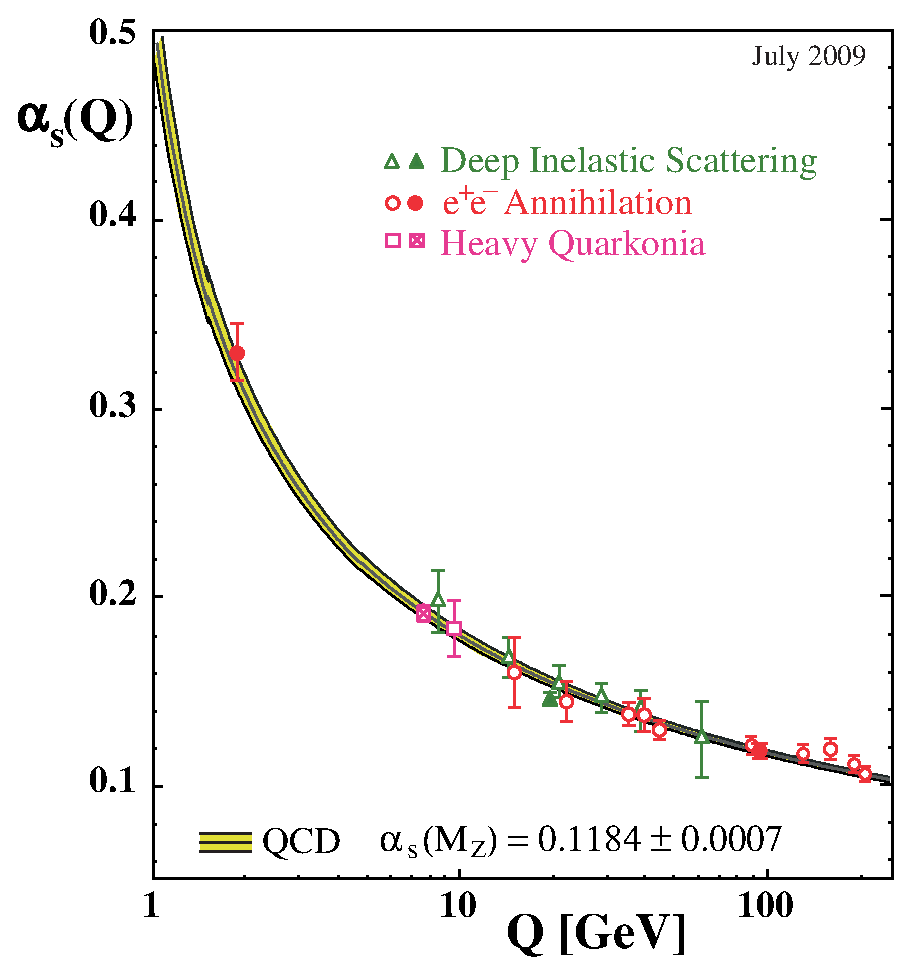
\includegraphics[width=0.795\textwidth]{StandardModel/Figures/asq-2009.eps}
    }
  \end{center}
  \caption[Measurement of $\alpha_s(Q)$~\cite{Bethke:2009jm}.]{Measurement of $\alpha_s(Q)$~\cite{Bethke:2009jm}.}
  \label{fig:alphaRunning}
\end{figure}

\begin{equation}
\mu_{R}^{2} \frac{d\alpha_s(\mu_{R}^{2})}{d\mu_{R}^{2}} = -(33 - 2n_{f})\alpha_{s}^{2}(\mu_{R}^{2}),
\label{eq:RGE_QCD}
\end{equation}

\noindent where $\alpha_{s}(\mu_R)$ is the coupling as a function of an (unphysical) renormalization scale $\mu_R$, and $n_f$ is the number of families or generations.

The minus sign in the previous equation has its origin in the gluon self-interaction and leads to the two main characteristic properties of QCD: \emph{asymptotic freedom} and \emph{confinement}.
The integration of Equation \ref{eq:RGE_QCD} shows that at very high energies or equivalently, at very short distances the strong interaction coupling is weak.
This situation is called asymptotic freedom and is totally supported by the results from deep inelastic scattering (DIS) experiments (described in the next section).
Therefore, inside hadrons, the quarks behave as almost being free particles. 
In the $\unit[100]{GeV}$-$\unit[1]{TeV}$ energy range, $\alpha_s\sim 0.1$, and perturbation theory can be applied to QCD (pQCD).

This equation also shows that the coupling constant asymptotically diverges at low energies (large distances), making therefore impossible to produce isolated quarks.
When in a $q\bar{q}$ pair, the quarks begin to separate from each other, the energy of the field between them increases.
At some point, it is energetically favorable to create an additional $q\bar{q}$ pair, so at the end, there are only colorless bound states (hadrons).
This situation is called color confinement and it is related to the process of jet formation (Section~\ref{subsec:HadronizationModels}).


\section{Deep Inelastic Scattering}
    \label{sec:DIS}

\subsection{Probing the proton}
    \label{subsec:ProvingProton}

Deep Inelastic Scattering (DIS) experiments have been performed since the 1960's to study the internal structure of nucleons.
Electrons with energies up to $\unit[20]{GeV}$ were sent against a target of hydrogen:

\begin{equation}
e + P \rightarrow e + X,
\label{eq:DISschema}
\end{equation}

\noindent where $P$ is the proton and $X$ is any hadronic final state (Figure~\ref{fig:DISexample}).

\begin{figure}[!t]
  \begin{center}
    \mbox{
        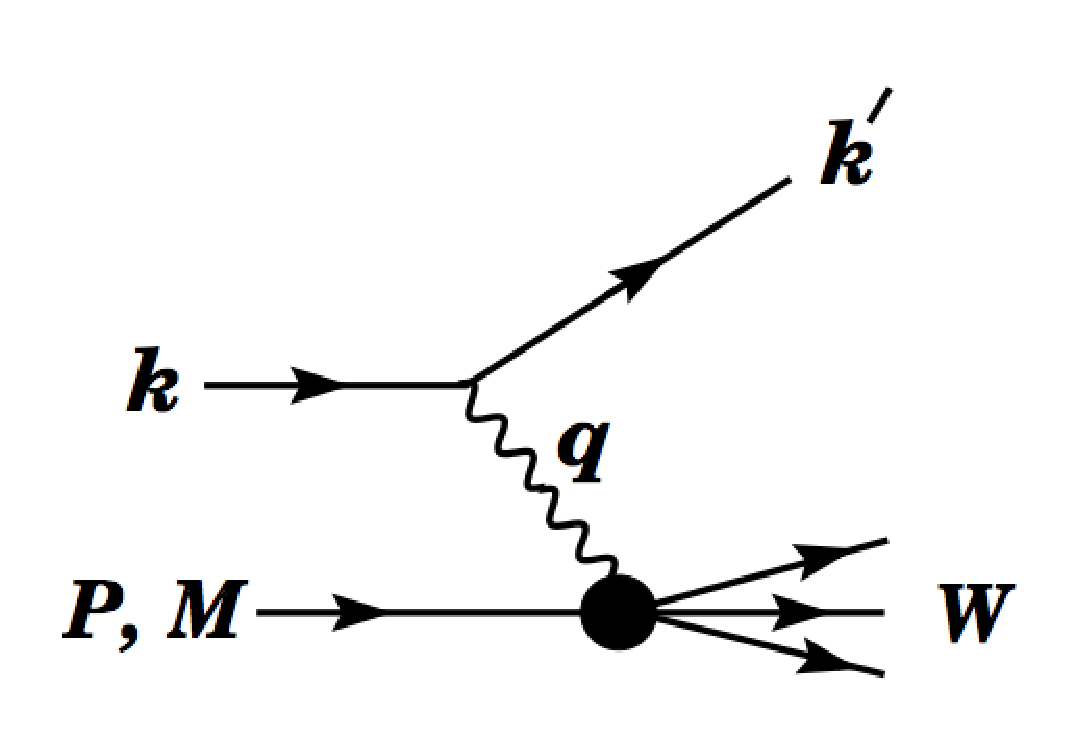
\includegraphics[width=0.495\textwidth]{StandardModel/Figures/DISexample.eps}
    }
  \end{center}
  \caption[Kinematic quantities for the description of the Deep Inelastic scattering.]{Kinematic quantities for the description of deep inelastic scattering. The quantities $k$ and $k'$ are the four-momenta of the incoming and outgoing leptons, $P$ is the four-momentum of a nucleon with mass $M$, and $W$ is the mass of the recoiling system $X$. The exchanged particle is a $\gamma$, $W^{\pm}$, or $Z$; it transfers four-momentum $q = k - k^{\prime}$ to the nucleon. \protect\cite{Beringer:1900zz}}
  \label{fig:DISexample}
\end{figure}

The kinematics of DIS can be described by the variables:

\begin{equation}
Q^2 \equiv -q^2 = (k-k')^2 \qquad\qquad x = \frac{Q^2}{2(P \cdot q)},
\label{eq:DISvariables}
\end{equation}

\noindent where $k$ and $k'$ are the four momentum of the incoming and outgoing electrons, $P$ is the momentum of the incoming proton and $x$ is interpreted as the fraction of the proton momentum carried by the interacting quark.

In the first DIS experiments, a larger number of large-angle deflected electrons than expected was found.
A phenomenological explanation to these results was given, considering the proton to be composed of non-interacting point-like particles, called \emph{partons}.
Therefore, $eP$ collisions can be regarded as ``hard'' interactions between the electron and partons inside the proton.
The Parton Model considers nucleons as bound states of three partons, each carrying a fraction $x$ of the total nucleon momentum such that:

\begin{equation}
\sum_{\text{partons}}{x_p} = 1.
\label{eq:sumFractionProton}
\end{equation}

In the parton model, the total cross section can be expressed in terms of electron-parton $ep$ interaction cross section:

\begin{equation}
\sigma(eP\rightarrow eX) = f \otimes \sigma(ep\rightarrow ep),
\label{eq:FactorizationTheoremSketch}
\end{equation}

\noindent where $f$ is the parton density, also called parton distribution function (PDF).
The term $f_i(x)dx$ gives the probability of finding a parton of type $i$ in the proton carrying a fraction between $x$ and $x+dx$ of the proton total momentum.
A prediction of the parton model is that, in the infinite-momentum frame of the proton, where $Q^2 \rightarrow \infty$ and the transverse momentum of the partons inside the proton are small, the parton densities are only a function of $x$.
This behavior is called Bjorken scaling.

However, in QCD, the radiation of gluons from the quarks leads to a violation of the scaling predicted by the Parton Model.
In particular, the DIS cross section can be written as:

\begin{equation}
\frac{d^2\,\sigma (e^{\pm}P)}{dx\,dQ^2} = \frac{4\pi\alpha^2}{xQ^4} \left( y^2 x F_1(x, Q^2) + (1-y) F_2(x, Q^2) \mp y(1-y)x F_3(x, Q^2) \right)
\label{eq:DISxsection}
\end{equation}

\noindent where $y = \frac{Q}{sx}$ and $F_i$ are the proton structure functions defined as:

\begin{equation}
F_1 = \frac{1}{2}\sum_i{e_i^2 f_i} \qquad \qquad F_2 = \frac{1}{2}\sum_i{e_i^2 x f_i},
\label{eq:DISformfactors}
\end{equation}

\noindent that explicitly depend on $Q$, and $F_3$ is found to be zero in parity conserving photon exchanges.
The reason for this dependence is that, an increase in $Q^2$ allows the gluons exchanged by the quarks (and their subsequent splittings into $q\bar{q}$ pairs) to be better resolved by the photon.
Figure~\ref{fig:ProtonPDFs} shows the parton distribution functions of a proton measured at different values of $Q^2$.
Valence quarks dominate for large values of $x$ (they carry the biggest fraction of the total proton momentum), while gluons and sea quarks dominate at low $x$. 
This figure also shows that as $Q^2$ increases, the probability for finding gluons and sea quarks at low $x$ values is higher.

\begin{figure}[!ht]
  \begin{center}
    \mbox{
        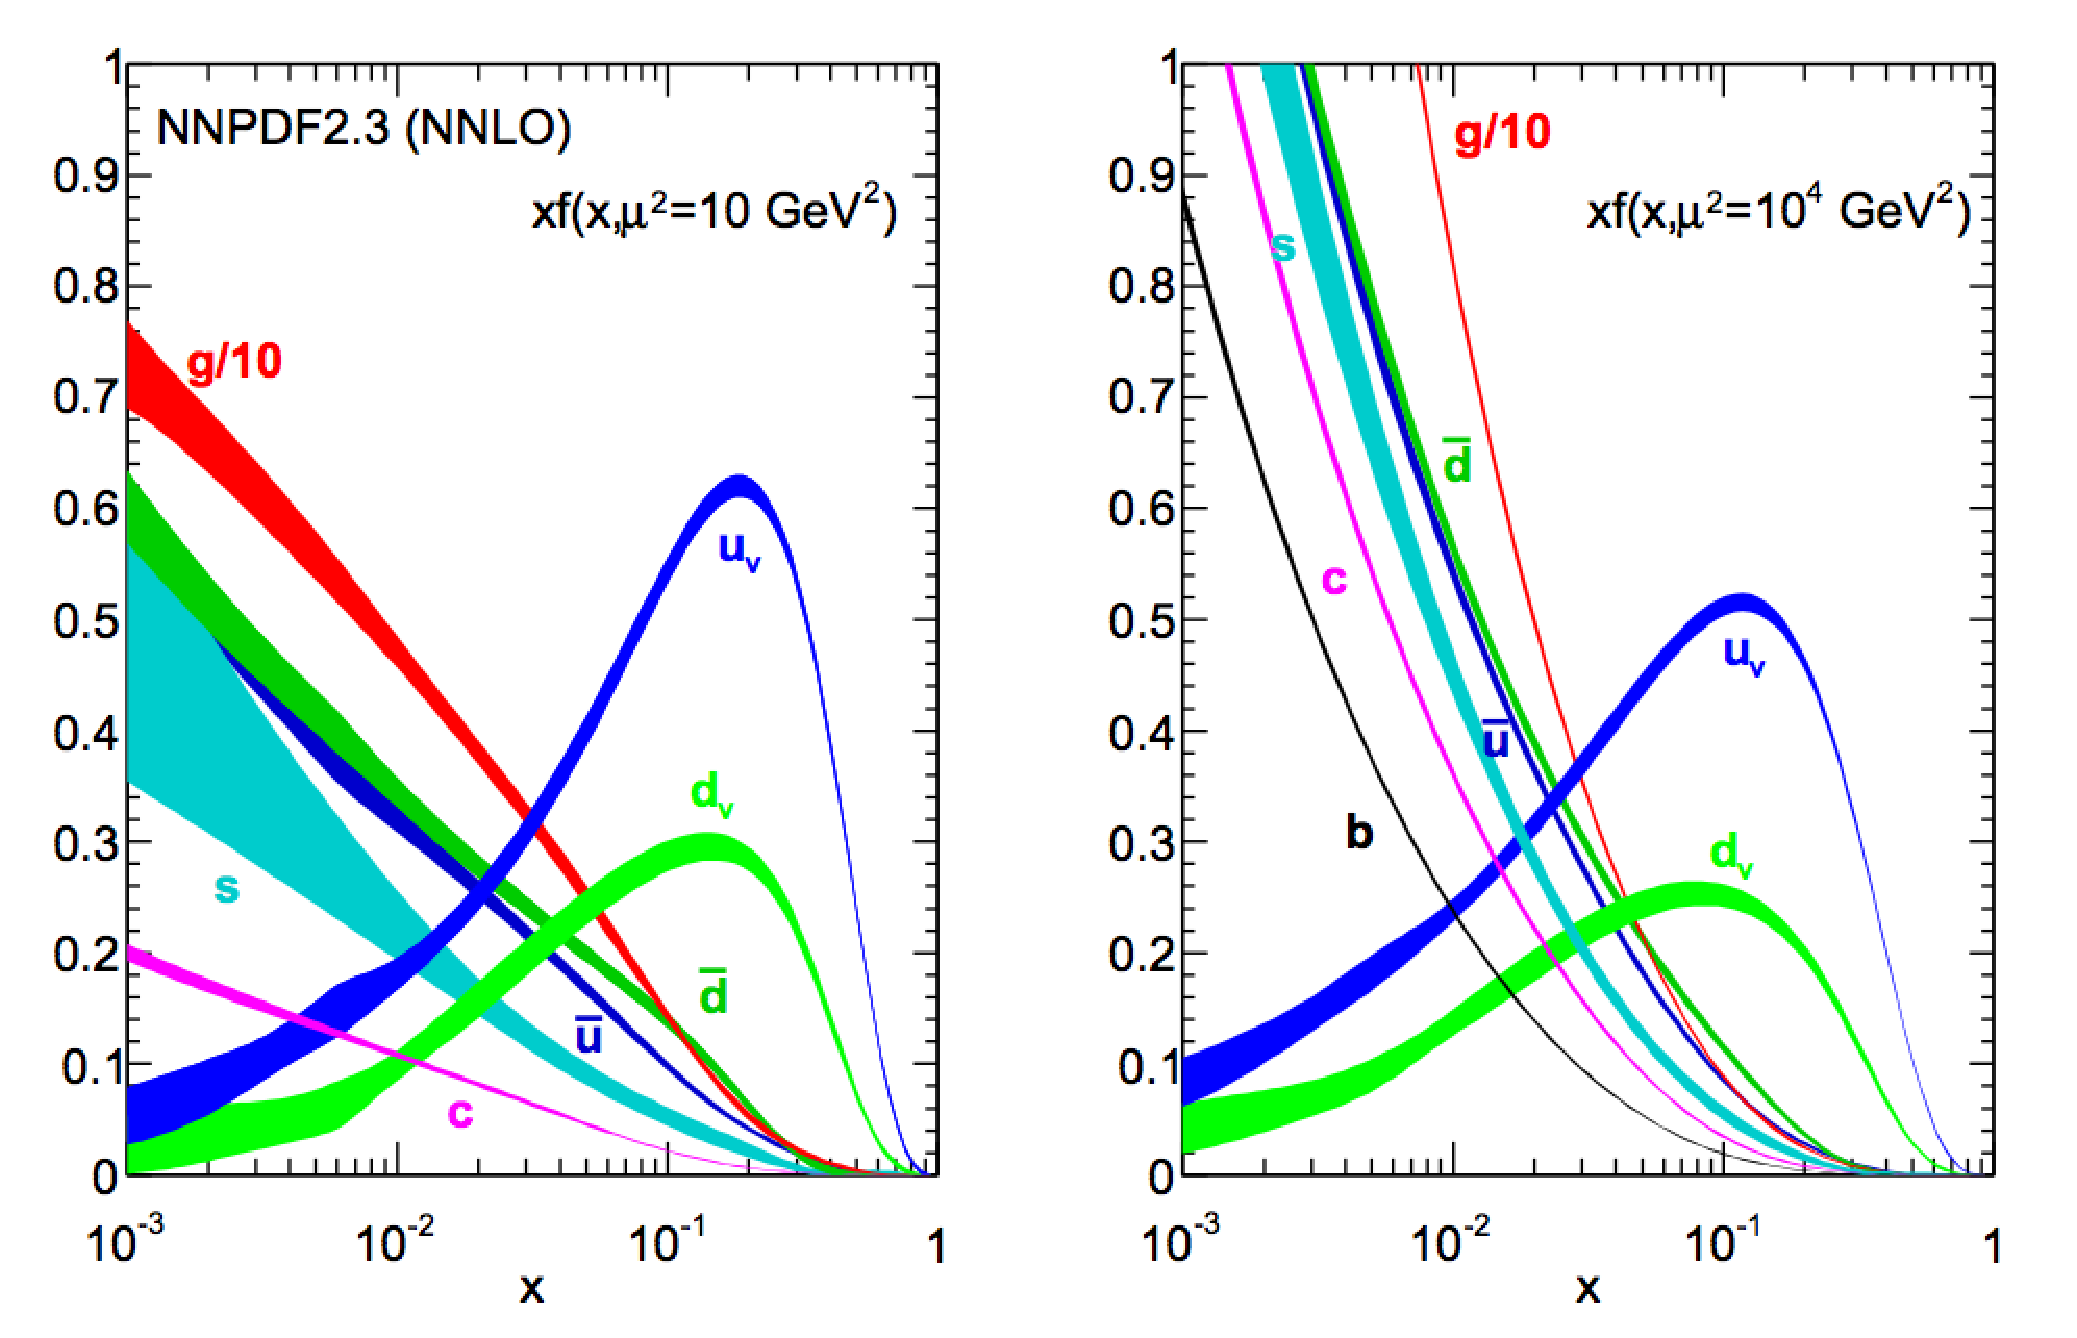
\includegraphics[width=0.995\textwidth]{StandardModel/Figures/ProtonPDF.eps}
    }
  \end{center}
  \caption[Distributions of the parton distribution functions $xf(x)$.]{Distributions of the parton distribution functions $xf(x)$ (where $f = u_v,\, d_v,\, \bar{u},\, \bar{d},\, s \approx \bar{s},\, c=\bar{c},\, b=\bar{b}$) obtained in NNLO \texttt{NNPDF2.3} global analysis at scales $\mu^2 = \unit[10]{GeV^2}$ and $\mu^2 = \unit[10^4]{GeV^2}$, with $\alpha_s(M_Z) = 0.118$. \protect\cite{Beringer:1900zz}}
  \label{fig:ProtonPDFs}
\end{figure}


\subsection{Parton Distribution Function}
    \label{subsec:PDF_proton}

The partonic description of the hadrons that are collided determines the theoretical predictions on high energy physics.
Perturbative QCD cannot predict the form of the PDFs, but can describe their evolution with the variation of the scale $Q^2$:

\begin{equation}
\begin{split}
\frac{d}{d\log{Q^2}}f_{q}(x, Q^2) = \frac{\alpha_s}{2\pi}\int_{x}^{1}{\frac{dy}{y}\,f_{q}(y, Q^2)\,P_{qq}\left(\frac{x}{y}\right) + f_{g}(y, Q^2)\,P_{qg}\left(\frac{x}{y}\right)} \\
\frac{d}{d\log{Q^2}}f_{g}(x, Q^2) = \frac{\alpha_s}{2\pi}\int_{x}^{1}{\frac{dy}{y}\,f_{q}(y, Q^2)\,P_{gq}\left(\frac{x}{y}\right) + f_{g}(y, Q^2)\,P_{gg}\left(\frac{x}{y}\right)}.
\end{split}
\label{eq:EvolutionPDF}
\end{equation}

\noindent where $P_{ab}(z)$ are the Dokshitzer-Gribov-Lipatov-Altarelli-Parisi (DGLAP) splitting functions, that describe the probability that a parton of type $b$ radiates a quark or a gluon of type $a$, carrying a fraction $z$ of the initial's parton momentum.
In particular, the first expression describes the change of the quark densities with $Q^2$ due to gluon radiation and gluon splitting, while the second expression describes the change of the gluon densities with $Q^2$ due to gluon radiation from quarks and gluons.
The DGLAP splitting functions at the lowest order in $\alpha_s$, in the small angle approximation and averaging over the polarizations and spins are expressed as~\cite{Halzen}:

\begin{equation}
\begin{split}
&P_{qq}(z) = \frac{4}{3}\frac{1+z^2}{1-z}, \\
&P_{gq}(z) = \frac{4}{3}\frac{1+(1-z)^2}{z}, \\
&P_{qg}(z) = \frac{1}{2}\left(z^2+(1-z)^2\right), \\
&P_{gg}(z) = 6\left(\frac{1-z}{z} + \frac{z}{1-z} + z(1-z)\right).
\end{split}
\label{eq:DGLAP}
\end{equation}


\subsection{PDF parametrization}

Experimental data are fitted to obtain the parton densities at a given scale $Q^2$, and the evolution equations \ref{eq:EvolutionPDF} are used to predict the PDFs at different scales.
Figure~\ref{fig:DIS_F2fit} shows the structure function $F_2$ as a function of $x$ and $Q^2$ as measured from DIS and fixed target experiments, and the evolution predicted with the DGLAP equations.
The structure function $F_2$ shows no dependence on $Q^2$ for large values of $x$.
However, as $x$ decreases, the effect of the gluons and sea quarks start to be important, thus violating the Bjorken scaling.

\begin{figure}[!t]
  \begin{center}
    \mbox{
        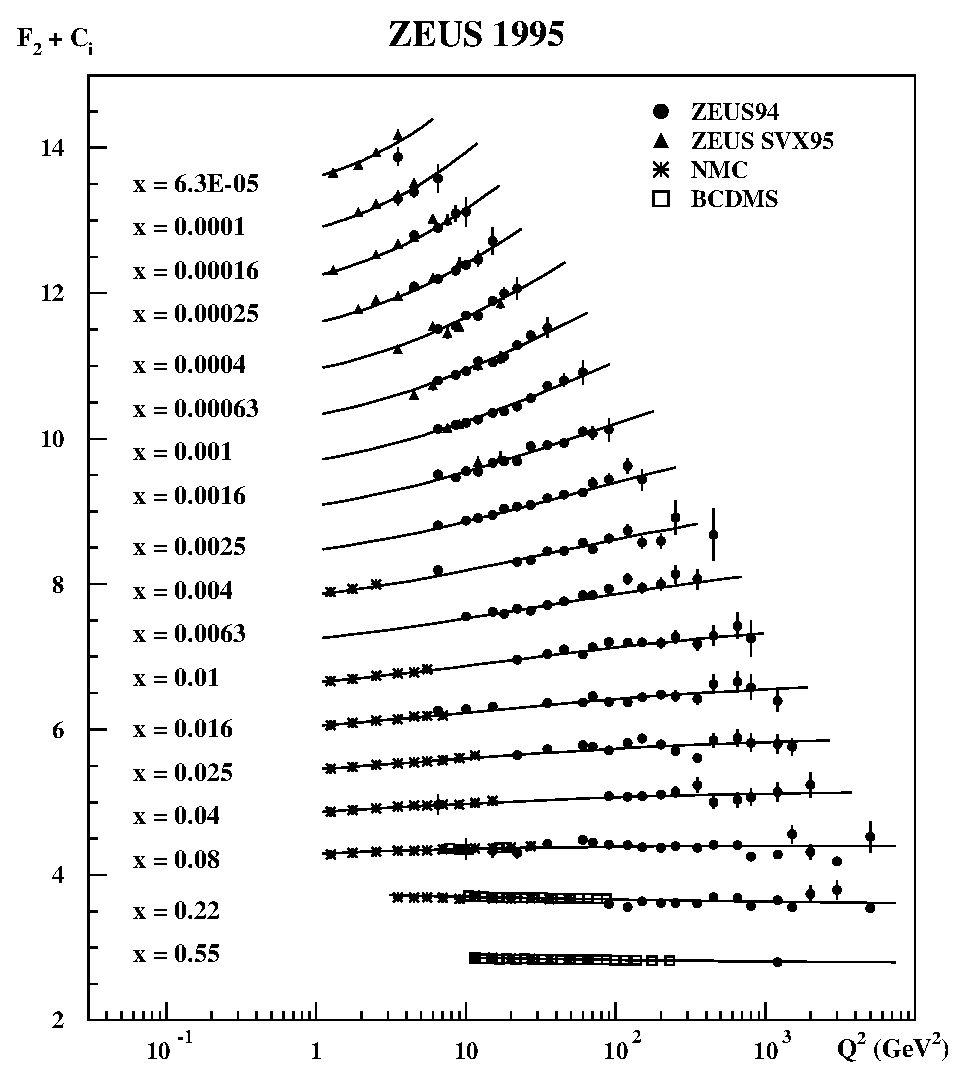
\includegraphics[width=0.995\textwidth]{StandardModel/Figures/StructureFunctionZEUS.eps}
    }
  \end{center}
  \caption[The proton structure function $F_2$ versus $Q^2$ at fixed values of $x$.]{The proton structure function $F_2$ versus $Q^2$ at fixed values of $x$. Data are from the ZEUS94 and SVX95 analyses and from the NMC and BCDMS fixed target experiments. For clarity an amount $C_i = 13.6-0.6i$ is added to $F_2$ where $i=1$ (18) for the lowest (highest) $x$ value~\cite{Breitweg:1998dz}.}
  \label{fig:DIS_F2fit}
\end{figure}

The PDFs are expected to be smooth functions of the scaling variable $x$, and can be parametrized.
In this analysis, the parametrization provided by the CTEQ~\cite{Lai:1994bb}, CT10~\cite{Lai:2010vv} and MSTW~\cite{Martin:2009iq} collaborations are used.
As an example, the CT10 parametrizaton used for the quarks and the gluon parton densities is:

\begin{equation}
xf_i(x, Q^2_0) = A_0 \cdot x^{A_1}(1-x)^{A_2}\exp{(A_3x + A_4 x^2 + A_5\sqrt{x})},
\label{eq:parametrizationPDF}
\end{equation}

\noindent where $f_i$ is a particular parton density at $Q^2_0$ and $A_i$ are the parameters to be fitted, obtained with a $\chi^2$ parametrization over data from different types of measurements.
Not all these parameters are free, since these functions must satisfy flavor and momentum sum rules.


\section{Monte Carlo simulation}
    \label{sec:MCSimulation}

Monte Carlo (MC) codes are tools that enable the description of the final states resulting from high-energy collisions, where the state-of-the-art knowledge about QED and QCD is implemented by using MC techniques.
They have been developed to help interpreting the data from high energy particle colliders in order to extract the measurement of fundamental physical parameters or to infer the possible existence of new physics beyond the SM.
The next subsections are devoted to describe the different phases of a MC event generation~\cite{Skands:2011pf,ellis2003qcd}.
Figure~\ref{fig:HardCollisionEvolution} shows the general structure of a hard proton-proton collision.
The dotted circle {\em H} separates the perturbative QCD (hard process, initial and final state radiation) from non-perturbative contributions (underlying event, hadronization and PDFs).
%Finally, a summary of the characteristics of the MC generators used in the analysis presented will be shown.

\begin{figure}[!ht]
  \begin{center}
    \mbox{
        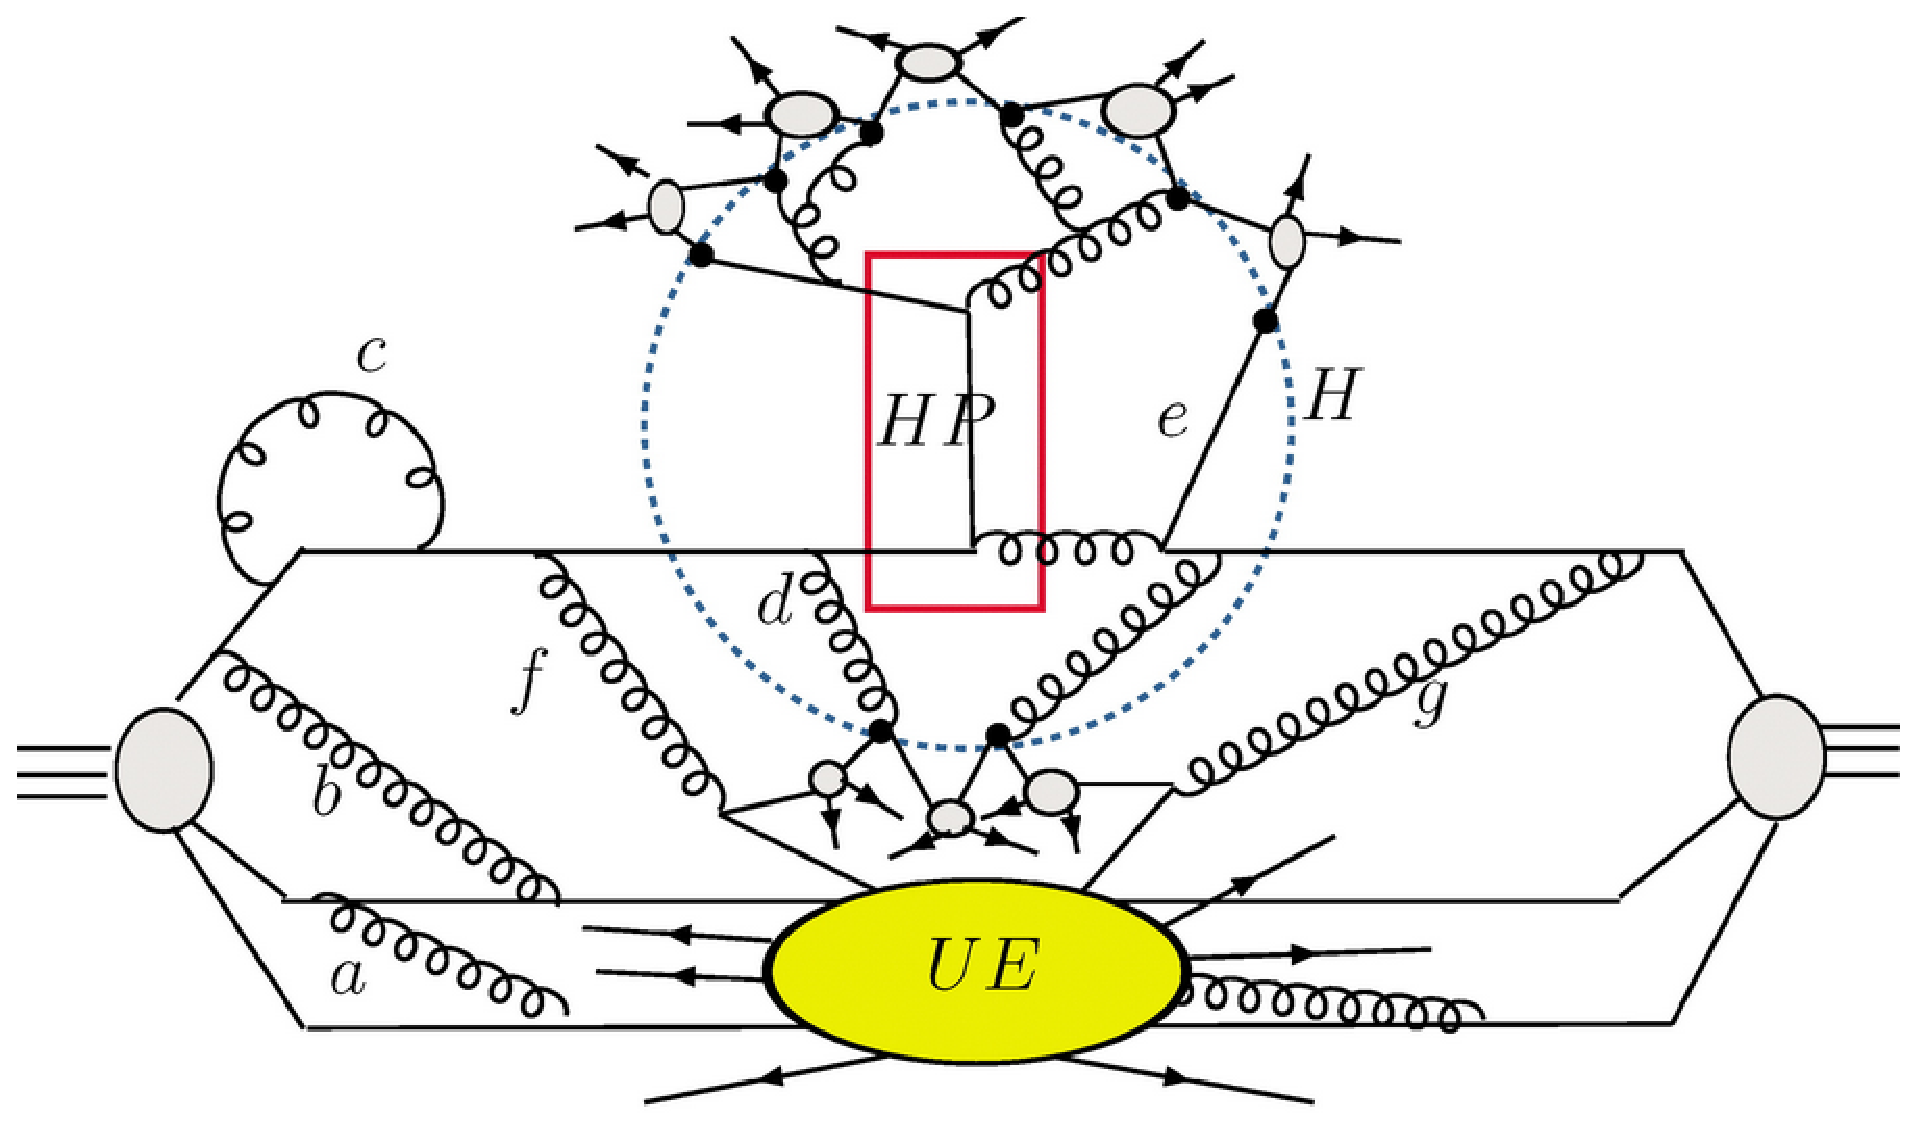
\includegraphics[width=0.995\textwidth]{StandardModel/Figures/HardInteractionEvolution.eps}
    }
  \end{center}
  \caption[General structure of a hard proton-proton collision.]{General structure of a hard proton-proton collision. HP, denotes the hard process, and UE, is the underlying event~\protect\cite{Mangano:2005dj}.}
  \label{fig:HardCollisionEvolution}
\end{figure}


\subsection{Parton-level event generators}
    \label{subsec:EventGenerators}

The cross section for a two-hadron interaction with momenta $P_1$ and $P_2$, can be factorized into short- and long-distance effects delimited by a factorization scale $\mu_F$, according to the factorization theorem:

\begin{equation}
\begin{split}
\sigma(P_1, P_2) = \sum_{i, j} \int dx_1\, dx_2\, f_i(x, \mu_F^2)\, f_j(x, \mu_F^2) \\
  \times\; \hat{\sigma}_{ij}(p_1, p_2, \alpha_s(\mu_R^2), Q^2/\mu_F^2,  Q^2/\mu_R^2) 
\end{split}
\label{eqXSecQCDComputation}
\end{equation}

\noindent where $f_i$ are the PDFs of each interacting parton, the sum runs over all parton types, and $\hat{\sigma}_{ij}$ is the parton cross section for incoming partons with momenta $p_1=x_1P_1$ and $p_2=x_2P_2$, respectively.
As long as the same factorization scale is used, the same PDFs extracted from DIS experiments can be used for $ep$, $\pp$ and $\ppbar$ experiments.
$\hat{\sigma}_{ij}$ is calculated at a given order on pQCD, which introduces a dependence on a renormalization scale $\mu_R$, that is usually chosen to be equal to $\mu_F$.

Schematically, the all-orders partonic cross section, $\hat{\sigma}_{ij}$ for a given process $F$, with any extra emission, can be expressed as:

\begin{equation}
\begin{split}
\hat{\sigma}_{ij} &= \int{d\mathcal{O}\; \frac{\hat{\sigma}_{ij}}{d\mathcal{O}}} \\
                  &= \int{d\mathcal{O}} \; \underbrace{\sum_{k=0}^{\infty}{\int{d\Phi_{F+k}}}}_{\Sigma\text{ legs}}
                                          |\underbrace{\sum_{\ell=0}^{\infty}{\mathcal{M}^{\ell}_{F+k}} }_{\Sigma \text{ loops}}|^2 \delta(\mathcal{O} - \mathcal{O}(\Phi_{F+k})) ,
\end{split}
\label{eq:AllOrdersXSection}
\end{equation}

\noindent where the sum over $k$ represents the sum over additional ``real emission'' corrections, called legs, and the sum over $\ell$ represents the sum over additional virtual corrections, loops.
$\Phi_{F+k}$ represents the phase space of the configuration with $k$ legs and $\ell$ loops.

The various fixed order truncations of pQCD can be recovered by limiting the nested sums in Equation~\ref{eq:AllOrdersXSection} to include only specific values of $k+\ell$.
Therefore,

\begin{itemize}
\item $k=0$, $\ell=0$: Leading order (usually tree-level) for inclusive $F$ production.
\item $k=n$, $\ell=0$: Leading order for $F+n$~jets.
\item $k+\ell \leq n$: N$^n$LO for $F$ (includes N$^{n-1}$LO for $F+1$ jet,  N$^{n-2}$LO for $F+2$ jets, and so on up to LO for $F+n$ jets).
\end{itemize}

The Kinoshita-Lee-Nauenberg (KLN) theorem~\cite{Kinoshita:1962ur,Lee:1964is} states that the divergences originated in the loops exactly cancel against those from the real emissions, order by order in perturbation theory.
However, in a fixed order calculation, e.g. leading order, in the situation for which $k\geq1, \ell=0$, the integration over the full momentum phase space will include configurations in which one or more of the $k$ partons become collinear or soft, thus leading to singularities in the integration region.
For this reason, the integration region needs to be modified to include only ``hard, well-separated'' momenta.
The remaining part of the phase space is then considered by the parton shower generators.


\subsection{Parton shower generators}
    \label{subsec:PartonShowerGenerators}

As already mentioned, the fixed order calculations introduced in the previous section are only valid if two conditions are fulfilled:

\begin{enumerate}
\item The strong coupling, $\alpha_s$, is small, so that perturbation theory is valid.
\item The phase space region is restricted to configurations in which real emissions are ``hard and well-separated''.
\end{enumerate}

Parton showers are included in the MC simulations to approximately account for the rest of higher order contributions to emulate a complete final state.
By the successive parton emission, the partons in the final state produce a cascade, where the splitting functions (Eq.~\ref{eq:DGLAP}) govern the radiation process.
A parton shower generator simulates the successive emission of quarks and gluons from the partons in the final (or initial) state.
This simulation is approximate, since it assumes completely independent parton emissions, neglects any interference term among them and does not consider virtual corrections.
In the almost-collinear splitting of a parton, the $n+1$-parton differential cross-section can be related to the $n$-parton cross section before splitting as

\begin{equation}
d\sigma_{n+1} \approx d\sigma_n \; dP_i(z,\mu^2)
\label{eq:PSrelation}
\end{equation}

\noindent where

\begin{equation}
dP_i(z,\mu^2) = \frac{d\mu^2}{\mu^2} \; \frac{\alpha_s}{2\pi} \; P_{ji}(z)dz 
\label{eq:dPi}
\end{equation}

\noindent shows the probability that parton $i$ will split into two partons at a virtuality scale $\mu$ and with parton $j$ carrying a fraction $z$ of the $i$'s parton momentum and $P_{ji}(z)$ are the same DGLAP equations from Eq. \ref{eq:DGLAP}.
This relation is universal, so for any process involving $n$ partons, this equation can be applied to obtain an approximation for $\sigma_{n+1}$.
This probability diverges logarithmically in the soft ($z=1, 0$) and collinear ($\mu = 0$) regions, which can be understood as a consequence of the non-perturbativity of QCD at low scales.
These divergences are not a problem because detectors will not be able to resolve two partons very close one another, thus introducing an effective cutoff to screen these regions.

The quality of the approximation from Equation~\ref{eq:dPi} is governed by how many terms besides the leading one shown in this equation are included.
Including all possible terms, the most general form for the cross section of the process $F + n$ jets, restricted to the phase-space region above some infrared cutoff scale, has the following algebraic structure:

\begin{equation}
\sigma_{F+n} = \alpha_s^n (\ln^{2n} + \ln^{2n-1} + \ln^{2n-2} + \cdots + \ln + \mathcal{R}),
\label{leadinglogapproximation}
\end{equation}

\noindent and therefore, the simplest approximation one can build from this equation is the ``leading-logarithmic'' (LL), in which all the terms of the series are dropped but the $\ln^{2n}$ one.

For the computer implementation of the parton shower, the Monte Carlo programs use Sudakov form factors:

\begin{equation}
\Delta_i(q_1^2, q_2^2) = \exp{\left( - \sum_{j} \int_{q_2^2}^{q_1^2}{\,\int_{z_\text{min}}^{z_\text{max}}{dP_i(z',dq'^2)}} \right)},
\label{eq:Sudakov}
\end{equation}

\noindent derived from the splitting functions.
The Sudakov form factors represent the probability that a parton evolves from an initial scale $q_1$ to a lower scale $q_2$ without branching.

To simplify the implementation of the calculations in the Monte Carlo programs, the radiations are separated into initial-state and final-state showers, depending on whether they start off an incoming or outgoing parton of the hard scattering.
In the final-state showers, the Monte Carlo branching algorithm operates in steps:

\begin{enumerate}
\item When a branching $a\rightarrow b + c$ occurs at scale $q_a$, the fraction of momentum carried by the daughter partons $x_b/x_a$ is determined using the appropriate splitting function $P_{ab}$, and the opening angle $\theta_a$ between $b$ and $c$ is given by $q_a = E_a^2(1-\cos{\theta_a})$.

\item The scale at which the partons $b$ and $c$ will branch is determined with the Sudakov factors.
Since the scale $q_a$ is proportional to the virtual mass, $q_b$ and $q_c$ are kinematically constrained to satisfy $\sqrt{q_a} > \sqrt{q_b} + \sqrt{q_c}$, thus imposing that the subsequent branchings on the daughter partons will have smaller opening angles.

\item The shower is terminated when these virtualities have fallen to the hadronization scale, $Q^2\sim\unit[1]{GeV}$.
\end{enumerate}

In the initial state showers, the same algorithm is applied, but operated backwards in time.
Starting from an incoming parton at the hard interaction $b$, it finds the branching $a\rightarrow b+c$, where $c$ can further branch in a final-state fashion.
Therefore, in the construction of the initial-state shower, the fraction of momentum $x$ is increased, and at the end it will match that described by the PDFs.


\subsection{Matrix element and parton shower matching}
    \label{subsec:MEandPSmatching}

The addition of the parton shower to the parton-level event generator can introduce double-counting of events in some regions of the phase space.
This is illustrated in a very simple way in Figure~\ref{fig:MatchingOverlap}.
The LO cross section for some process (green area), $F$, with a LL shower added to it (yellow area), is found in the left-pane of this figure.
To improve the description of the $F+1$ process from LL to LO, one needs to add the actual LO matrix element for $F+1$ (with a LL parton shower description as well).
However, the LO matrix element for $F+1$ is divergent, and therefore, only the phase-space region with at least one hard resolved jet can be covered (illustrated by the half shaded boxes in the middle pane of Figure~\ref{fig:MatchingOverlap}).
When one adds these two samples, the LL terms of the inclusive cross section for $F+1$ are counted twice, once from the shower of $F$, and once from the matrix element for $F+1$, illustrated by the red areas of the right-hand pane of Figure~\ref{fig:MatchingOverlap}.

\begin{figure}[!ht]
  \begin{center}
    \mbox{
        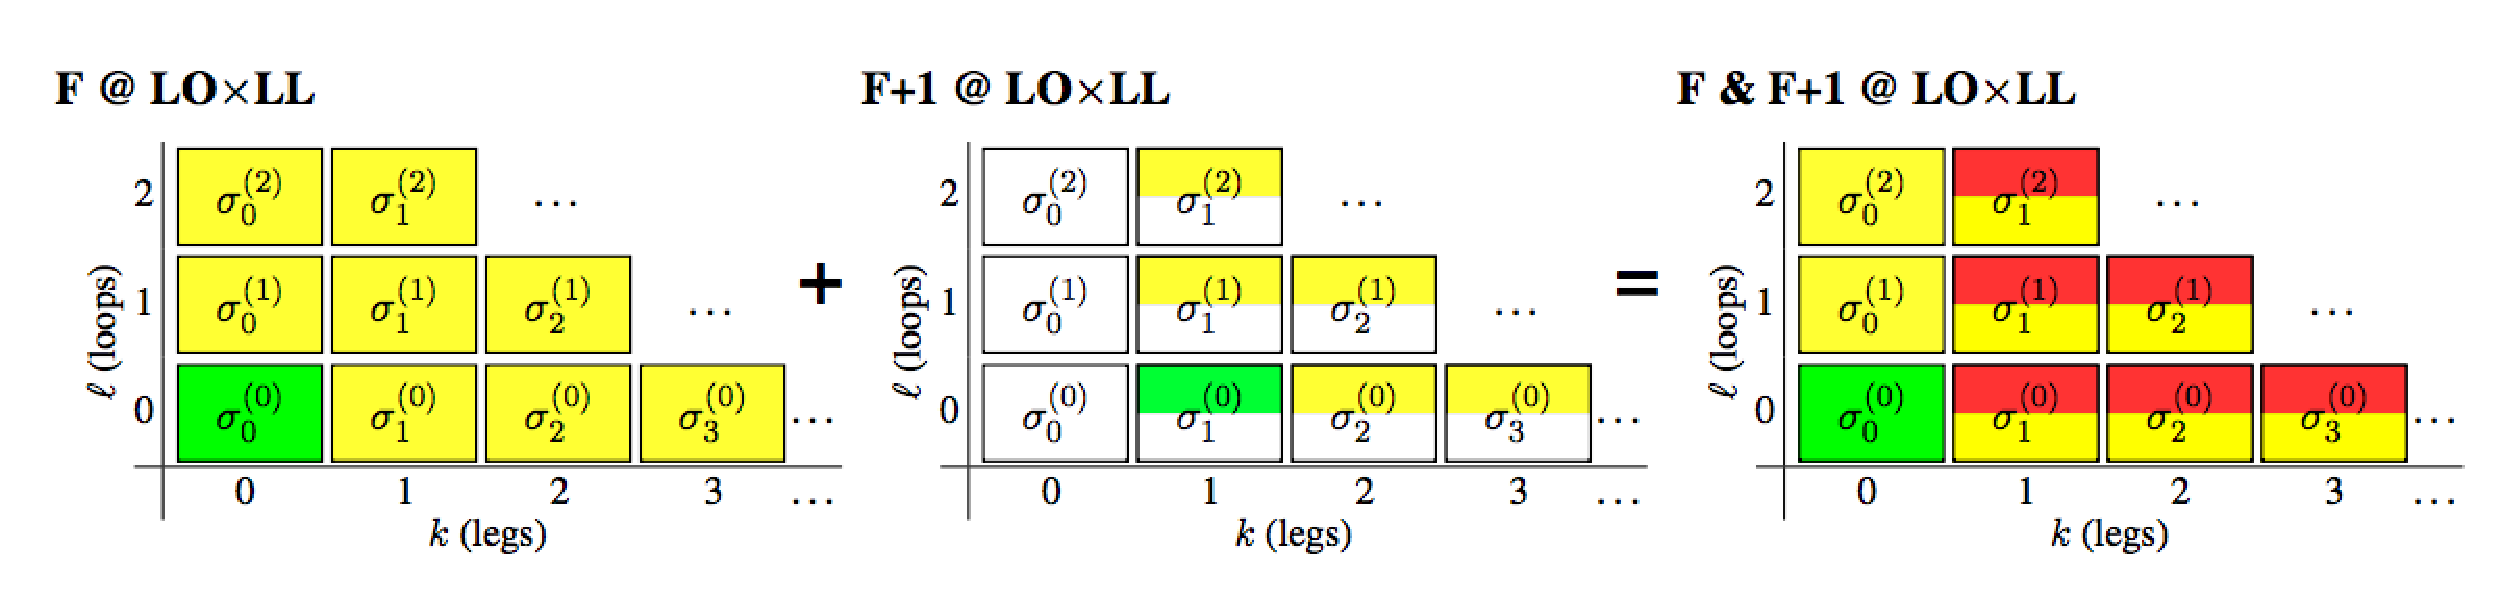
\includegraphics[width=0.995\textwidth]{StandardModel/Figures/MatchingMCOverlap.eps}
    }
  \end{center}
  \caption[Double-counting problem caused by adding cross sections involving matrix elements with different numbers of legs]
{Illustration of the double-counting problem caused by naively adding cross sections involving matrix elements with different numbers of legs~\cite{Skands:2011pf}.}
  \label{fig:MatchingOverlap}
\end{figure}

To remove this overlap, the phase space covered by the matrix element calculation, and the space covered by the parton shower evolution needs to be separated.
There are two main matching schemes: the Catani-Krauss-Kuhn-Webber (CKKW \cite{Catani:2001cc}) and the Michelangelo L. Mangano (MLM \cite{Mangano:2006rw}) methods.
They separate the phase space into the ME and PS regions by introducing resolution parameters that distinguish between resolved and non-resolved jets, to be described by the ME and the PS, respectively.

In the CKKW algorithm, a parton branching history is generated using the \kt{} algorithm \cite{Catani:1991hj}, given a configuration with $n$ partons in the final state.
The values of $\alpha_s$ in every vertex of the branching, and the Sudakov factor from every line between the vertices, are used to reweight the matrix elements.
The initial conditions of the shower are then set to have a smooth transition between the reweighted matrix elements and the parton shower, where the hard emissions in the shower evolution are vetoed if they have enough transverse momentum to produce a separate jet, according to the \kt{} algorithm.

The matching MLM procedure starts by separating the events in exclusive samples of $n$ partons in the final state, and then, the parton shower is developed in that event using a PS Monte Carlo.
The parton configuration after the showering is then processed with a cone jet algorithm, with a radius $R_{\text{jet}}$.
Then, the original $n$ partons are matched to the jets if $\Delta R(\text{jet}, \text{parton}) < R_{\text{jet}}$.
If all the partons are matched to a jet and there are no extra jets, i.e. $N_{\text{jets}}=n$, the event is accepted.
Otherwise, the event is rejected to avoid further hard emissions that would lead to additional jets.
Finally, the events with different jet multiplicities, $n=0, 1, 2, \ldots, k$, are recombined in a single sample.
The events in the sample with parton multiplicities higher than $k$ jets are accepted if $N_\text{jets}\geq k$.


\subsection{Hadronization models}
    \label{subsec:HadronizationModels}

As the collision process evolves and the partons radiate and travel further apart, the QCD running coupling increases as the values of the shower evolution scale $Q^2$ decrease.
Therefore, the confining effects of QCD become important and the dynamics enter a non-perturbative phase which leads to the formation of the observed final-state hadrons.
Event generators have to rely on models based on general features of QCD.

As a consequence of the factorization assumption and color preconfinement, the hadronization of the partons is independent of the hard scattering process.
Therefore, the parameters of a model used to describe a hadronization can be fitted to the results of one experiment and then applied to another.

The most used hadronization models are the string fragmentation and the cluster hadronization models, which are described below.

\begin{figure}[!ht]
  \begin{center}
    \mbox{
        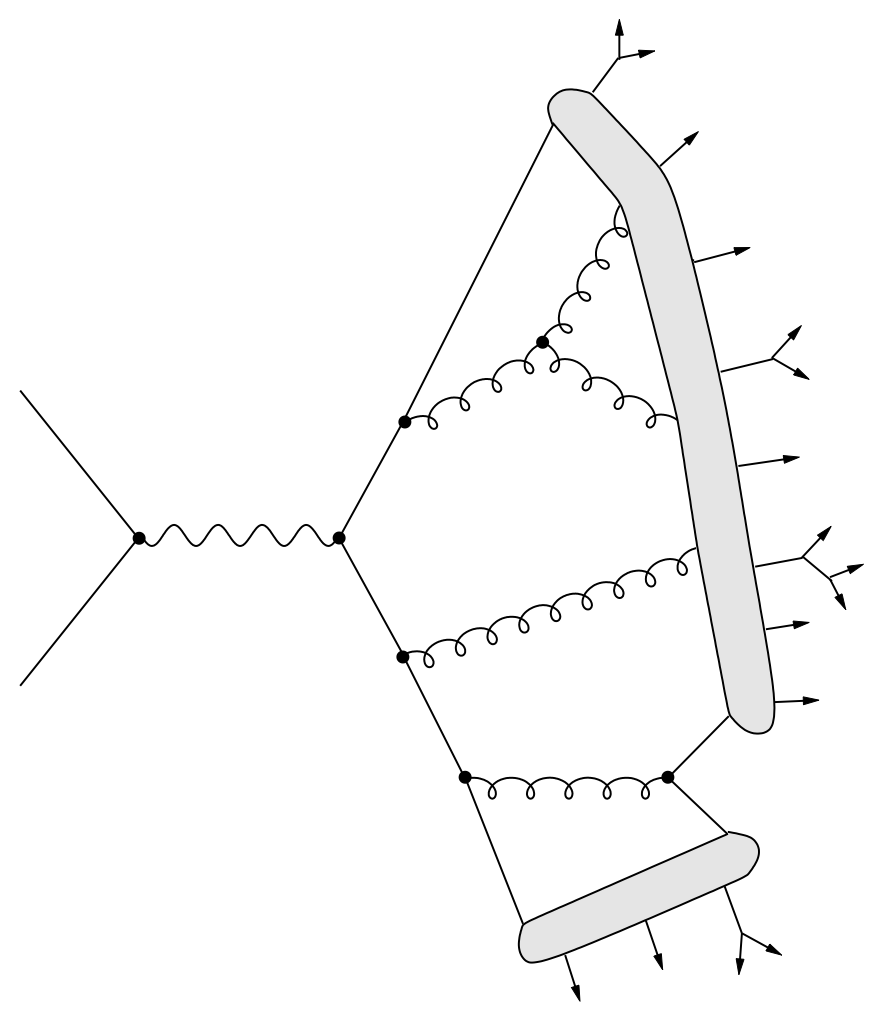
\includegraphics[width=0.495\textwidth]{StandardModel/Figures/HadronizationString.eps}
        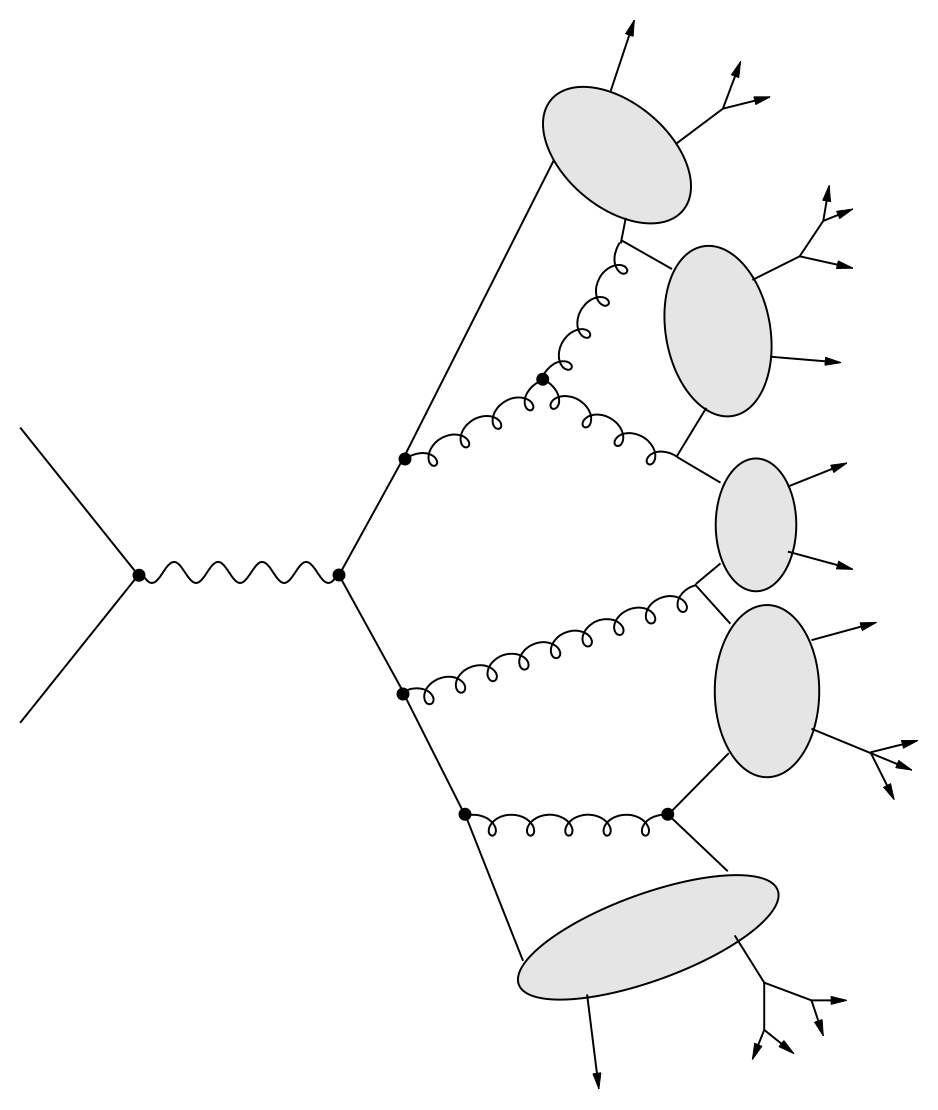
\includegraphics[width=0.495\textwidth]{StandardModel/Figures/HadronizationCluster.eps}
    }
  \end{center}
  \caption[Illustration of different hadronization models.]{Illustration of string fragmentation (left) and cluster hadronization (right) \protect\cite{Ellis:1991qj}.}
  \label{fig:HadronizationModels}
\end{figure}


\subsubsection{String fragmentation hadronization model}
    \label{subsubsec:StringModel}

The string model for hadronizaton, schematically shown in Figure \ref{fig:HadronizationModels} (left), uses string dynamics to describe the flux between a $q\bar{q}$ pair.
It is based on the observation that at large distances the potential energy of color sources increases linearly with their separation.
In the evolution of the hadronization process, the potential energy of the string increases as partons travel further apart at the expense of its kinetic energy.
When this energy becomes higher than the mass of a light $q\bar{q}$ pair, a new $q'\bar{q}'$ is created and the string breaks into two shorter strings creating two color-singlet states $q'\bar{q}$ and $q\bar{q}'$.
If the relative momentum of the new $q\bar{q}$ pairs connected to the same string is large enough, the string might break again.
Gluons act as ``kinks'' in the string, that add extra tension to it.
The creation of heavy quarks is suppressed during the hadronization as the production of light quark pairs ($u$, $d$ and $s$) is more energy favored.
The formation of baryons, 3-quark states, is achieved by considering them quark-diquark states, where diquarks are simply treated as antiquarks.


\subsubsection{Cluster hadronization model}
    \label{subsubsec:ClusterModel}

The cluser model is based on the color pre-confinement of the branching processes.
The process starts by splitting gluons that remain after parton shower into quark-antiquark pairs, so that only quarks are present.
They are then grouped in color-singlets.
The mass spectrum of these clusters peaks at low values of the order of the GeV, but has a broad tail at high masses.
The clusters decay typically into two hadrons.
Heavier hadrons are naturally suppressed by the mass spectra.
Furthermore, the heaviest clusters can decay into smaller clusters that subsequently decay into hadrons.
A sketch of this model is shown in Figure \ref{fig:HadronizationModels} (right).


\subsection{Underlying event}
    \label{subsec:UnderlyingEvent}

The underlying event (UE) refers to the interactions involving partons that do not directly take part in the hard scattering.
It cannot be described perturbatively because the interactions happen at low transferred momentum. 
These interactions also involve flavor and color connections to the hard scattering, and therefore they cannot be separated from the hard scattering in general.
The presence of particles originated in the UE can affect the interpretation of the data, for example, by contributing to the energy associated to the jets.
Phenomenological models~\cite{Butterworth:1996zw} are used to simulate the UE and are tuned to minimum bias data from hadron colliders~\cite{Sjostrand:2006za}.


\subsection{Monte Carlo generators}
    \label{subsec:MCgenerators}

A summary of the different MC generators used in this Thesis is presented in Table~\ref{tab:MCgenSummary}, and briefly discussed in the following sections~\cite{Buckley:2011ms, Aad:2010ah}.

\begin{table}[!ht]
  \begin{center}
    \begin{small}
      \setlength{\tabcolsep}{0.0pc}
      \begin{tabular*}{\textwidth}{@{\extracolsep{\fill}}ccccc}
        \noalign{\smallskip}\hline\hline\noalign{\smallskip}
        \textbf{Monte} & \textbf{Matrix}  & \textbf{ISR/} & \multirow{2}{*}{\textbf{Hadronization}} & \textbf{Underlying} \\
        \textbf{Carlo} & \textbf{element} & \textbf{FSR}  &                                         & \textbf{event} \\
        \noalign{\smallskip}\hline\noalign{\smallskip}
        \pythia{}      & LO               & Parton shower & String model  & Minimum bias \\
        \herwig{}      & LO               & Parton shower & Cluster model & \jimmy{}  \\
        \multirow{2}{*}{\sherpa{}}      & \multirow{2}{*}{LO}               & \pythia{}     & \multirow{2}{*}{\pythia{}}     & \multirow{2}{*}{\pythia{}} \\
         & & (CKKW matching)& & \\
        \multirow{3}{*}{\alpgen{}}      & \multirow{3}{*}{LO}               & \pythia{} or   & \multirow{3}{*}{\pythia{}}     & \multirow{3}{*}{\pythia{}} \\
         & & \herwig{}& & \\
         & & (MLM matching)& & \\
        \mcnlo{}       & NLO              & \herwig{} & \herwig{} & \herwig{} (\jimmy{})\\
        \multirow{2}{*}{\powheg{}}      & \multirow{2}{*}{NLO}               & \pythia{} or     & \pythia{} or     & \pythia{} or \\
         & & \herwig{} & \herwig{} & \herwig{} \\
        \multirow{2}{*}{\acer{}}      & \multirow{2}{*}{LO}               & \pythia{} or     & \pythia{} or     & \pythia{} or \\
         & & \herwig{} & \herwig{} & \herwig{} \\
        \multirow{2}{*}{\madgraph{}}      & \multirow{2}{*}{LO}               & \pythia{}     & \multirow{2}{*}{\pythia{}}    & \multirow{2}{*}{\pythia{}} \\
           & & (MLM matching) & &  \\
        \noalign{\smallskip}\hline\hline\noalign{\smallskip}
      \end{tabular*}
    \end{small}
  \end{center}
  \caption[Summary of the Monte Carlo generators used in the analysis.]{Summary of the Monte Carlo generators used in the analysis.}
  \label{tab:MCgenSummary}
\end{table}


\subsubsection{General purpose Monte Carlo generators}

\pythia{}~\cite{Sjostrand:2006za} and \herwig{}~\cite{Corcella:2000bw,Bahr:2008dy} are general purpose event generators that use matrix elements at leading-order in perturbation theory in QCD.
They are optimized to compute 2-to-1 and 2-to-2 processes, although 2-to-$n$ ($n>2$) processes can be achieved with initial- and final-state radiation, ordered in $\pt$ (angle) in the case of \pythia{} (\herwig{}).
For hadronization, \pythia{} uses the string model, while the cluster model is used in \herwig{}.
The latest is normally interfaced with \jimmy{}~\cite{Butterworth:1996zw} to model the underlying event. 


\subsubsection{Multi-leg Monte Carlo generators}

\sherpa{} \cite{Gleisberg:2008ta}, \alpgen{} \cite{Mangano:2002ea} and \madgraph{} \cite{Alwall:2011uj} are multi-purpose event generators, specialized in the computation of matrix elements involving 2-to-$n$ processes at LO in pQCD.
\madgraph{} and \alpgen{} compute separated ME up to $n=6$ and $n=9$, respectively.

In \sherpa{} the different jet multiplicities are generated in a single inclusive sample directly.
Parton showers and hadronizations are performed with either \pythia{} or \herwig{} for \alpgen{} and \sherpa{}, while \madgraph{} needs to be interfaced with \pythia{}.
The ME/PS matching is performed with the CKKW scheme in \sherpa{}, and with the MLM scheme in \alpgen{} and \madgraph{}.
Finally, \alpgen{} and \madgraph{} use \pythia{} to simulate the UE, while \sherpa{} uses its own implementation, closely following following the \pythia{} implementation.

In the analysis presented in the following chapters, \sherpa{} and \alpgen{} MC generators are used to model the $W/Z$+jets and the dibosons ($WW$, $ZZ$ or $WZ$) Standard Model processes.
The \madgraph{} interface, is instead used for the implementation of the new physics models.


\subsubsection{Next-to-leading order Monte Carlo generators}

\mcnlo{} \cite{Frixione:2008ym} and \powheg{} \cite{Frixione:2007vw} are event generators that use matrix elements at NLO in pQCD.
In the analysis, they are used to simulate processes involving the production of a top quark. 
\powheg{} is interfaced with either \pythia{} or \herwig{} for the modeling of the PS, hadronization or UE, while \mcnlo{} is interfaced with \herwig{}.
